\documentclass{ctexart}
\usepackage{avanti-color}
%\usepackage{avanti-font}
\usepackage{avanti-math}
\usepackage{avanti-theorem}
\usepackage{avanti-others}

\everymath{\color{black}}
\pagestyle{empty} % 没有页眉和页脚

 % define the plot style and the axis style
\tikzset{font=\Huge}
\definecolor{base01}{RGB} {088, 110, 117}
\definecolor{base}{RGB} {131, 148, 150}
\tikzset{arrow/.style={-,black}}
\tikzset{global scale/.style={
    scale=#1,
    every node/.append style={scale=#1}
  }
}
\begin{document}

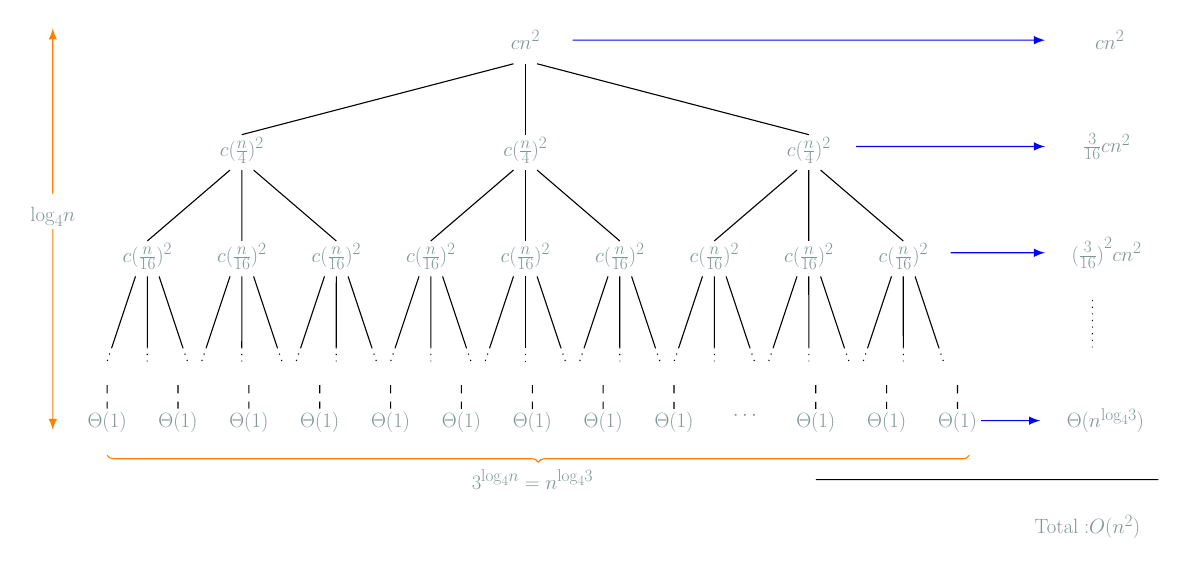
\begin{tikzpicture}[global scale = 0.3]
    \path (0,0) coordinate (O);
    \path [base] (O) node [above] () {$cn^2$};
    
    \path (O) ++(0,-0.5) coordinate (O);
    \path (O) ++(-12,-3) coordinate (O2);
    \path (O) ++(0,-3) coordinate (O3);
    \path (O) ++(12,-3) coordinate (O4);
    
    \path (O) ++(-0.5,0) coordinate (O11);
    \path (O) ++(0.5,0) coordinate (O12);
    
    \draw [arrow]  (O11) -- (O2);
    \draw [arrow]  (O) -- (O3);
    \draw [arrow]  (O12) -- (O4);

    \path [base] (O2) node [below] () {$c(\frac{n}{4})^2$};
    \path [base] (O3) node [below] () {$c(\frac{n}{4})^2$};
    \path [base] (O4) node [below] () {$c(\frac{n}{4})^2$};

    \path (O2) ++(0,-1.5) coordinate(O2);
    \path (O2) ++(-0.5,0) coordinate (O21);
    \path (O2) ++(0.5,0) coordinate (O22);
    
    \path (O2) ++(-4,-3) coordinate (O5);
    \path (O2) ++(0,-3) coordinate (O6);
    \path (O2) ++(4,-3) coordinate (O7);

    \draw [arrow]  (O21) -- (O5);
    \draw [arrow]  (O2) -- (O6);
    \draw [arrow]  (O22) -- (O7);

    \path (O3) ++(0,-1.5) coordinate(O3);
    \path (O3) ++(-0.5,0) coordinate (O31);
    \path (O3) ++(0.5,0) coordinate (O32);
    
    \path (O3) ++(-4,-3) coordinate (O8);
    \path (O3) ++(0,-3) coordinate (O9);
    \path (O3) ++(4,-3) coordinate (O10);

    \draw [arrow]  (O31) -- (O8);
    \draw [arrow]  (O3) -- (O9);
    \draw [arrow]  (O32) -- (O10);

    \path (O4) ++(0,-1.5) coordinate(O4);
    \path (O4) ++(-0.5,0) coordinate (O41);
    \path (O4) ++(0.5,0) coordinate (O42);
    
    \path (O4) ++(-4,-3) coordinate (O11);
    \path (O4) ++(0,-3) coordinate (O12);
    \path (O4) ++(4,-3) coordinate (O13);

    \draw [arrow]  (O41) -- (O11);
    \draw [arrow]  (O4) -- (O12);
    \draw [arrow]  (O42) -- (O13);

    \path [base] (O5) node [below] () {$c(\frac{n}{16})^2$};
    \path [base] (O6) node [below] () {$c(\frac{n}{16})^2$};
    \path [base] (O7) node [below] () {$c(\frac{n}{16})^2$};
    \path [base] (O8) node [below] () {$c(\frac{n}{16})^2$};
    \path [base] (O9) node [below] () {$c(\frac{n}{16})^2$};
    \path [base] (O10) node [below] () {$c(\frac{n}{16})^2$};
    \path [base] (O11) node [below] () {$c(\frac{n}{16})^2$};
    \path [base] (O12) node [below] () {$c(\frac{n}{16})^2$};
    \path [base] (O13) node [below] () {$c(\frac{n}{16})^2$};

    \path (O5) ++(0,-1.5) coordinate(O5);
    \path (O5) ++(-0.5,0) coordinate (O51);
    \path (O5) ++(0.5,0) coordinate (O52);
    
    \path (O51) ++(-1,-3) coordinate (O14);
    \path (O5) ++(0,-3) coordinate (O15);
    \path (O52) ++(1,-3) coordinate (O16);

    \draw [arrow]  (O51) -- (O14);
    \draw [arrow]  (O5) -- (O15);
    \draw [arrow]  (O52) -- (O16);

    \path (O6) ++(0,-1.5) coordinate(O6);
    \path (O6) ++(-0.5,0) coordinate (O61);
    \path (O6) ++(0.5,0) coordinate (O62);
    
    \path (O61) ++(-1,-3) coordinate (O17);
    \path (O6) ++(0,-3) coordinate (O18);
    \path (O62) ++(1,-3) coordinate (O19);

    \draw [arrow]  (O61) -- (O17);
    \draw [arrow]  (O6) -- (O18);
    \draw [arrow]  (O62) -- (O19);



    \path (O7) ++(0,-1.5) coordinate(O7);
    \path (O7) ++(-0.5,0) coordinate (O71);
    \path (O7) ++(0.5,0) coordinate (O72);

    \path (O71) ++(-1,-3) coordinate (O20);
    \path (O7) ++(0,-3) coordinate (O21);
    \path (O72) ++(1,-3) coordinate (O22);

    \draw [arrow]  (O71) -- (O20);
    \draw [arrow]  (O7) -- (O21);
    \draw [arrow]  (O72) -- (O22);

    \path (O8) ++(0,-1.5) coordinate(O8);
\path (O8) ++(-0.5,0) coordinate(O81);
\path (O8) ++(0.5,0) coordinate(O82);

\path (O81) ++(-1,-3) coordinate(O23);
\path (O8) ++(0,-3) coordinate(O24);
\path (O82) ++(1,-3) coordinate(O25);

\draw (O81) --(O23);
\draw (O8) --(O24);
\draw (O82) --(O25);

\path (O9) ++(0,-1.5) coordinate(O9);
\path (O9) ++(-0.5,0) coordinate(O91);
\path (O9) ++(0.5,0) coordinate(O92);

\path (O91) ++(-1,-3) coordinate(O26);
\path (O9) ++(0,-3) coordinate(O27);
\path (O92) ++(1,-3) coordinate(O28);

\draw (O91) --(O26);
\draw (O9) --(O27);
\draw (O92) --(O28);

\path (O10) ++(0,-1.5) coordinate(O10);
\path (O10) ++(-0.5,0) coordinate(O101);
\path (O10) ++(0.5,0) coordinate(O102);

\path (O101) ++(-1,-3) coordinate(O29);
\path (O10) ++(0,-3) coordinate(O30);
\path (O102) ++(1,-3) coordinate(O31);

\draw (O101) --(O29);
\draw (O10) --(O30);
\draw (O102) --(O31);

\path (O11) ++(0,-1.5) coordinate(O11);
\path (O11) ++(-0.5,0) coordinate(O111);
\path (O11) ++(0.5,0) coordinate(O112);

\path (O111) ++(-1,-3) coordinate(O32);
\path (O11) ++(0,-3) coordinate(O33);
\path (O112) ++(1,-3) coordinate(O34);

\draw (O111) --(O32);
\draw (O11) --(O33);
\draw (O112) --(O34);

\path (O12) ++(0,-1.5) coordinate(O12);
\path (O12) ++(-0.5,0) coordinate(O121);
\path (O12) ++(0.5,0) coordinate(O122);

\path (O121) ++(-1,-3) coordinate(O35);
\path (O12) ++(0,-3) coordinate(O36);
\path (O122) ++(1,-3) coordinate(O37);

\draw (O121) --(O35);
\draw (O12) --(O36);
\draw (O122) --(O37);

\path (O13) ++(0,-1.5) coordinate(O13);
\path (O13) ++(-0.5,0) coordinate(O131);
\path (O13) ++(0.5,0) coordinate(O132);

\path (O131) ++(-1,-3) coordinate(O38);
\path (O13) ++(0,-3) coordinate(O39);
\path (O132) ++(1,-3) coordinate(O40);

\draw (O131) --(O38);
\draw (O13) --(O39);
\draw (O132) --(O40);

\path (O14) ++(-.2,-.6)  coordinate(O41);
\path (O15) ++(0,-.6)  coordinate(O42);
\path (O16) ++(0.2,-.6)  coordinate(O43);

\draw[dotted] (O14) --(O41);
\draw[dotted] (O15) --(O42);
\draw[dotted] (O16) --(O43);

\path (O17) ++(-.2,-.6)  coordinate(O44);
\path (O18) ++(0,-.6)  coordinate(O45);
\path (O19) ++(.2,-.6)  coordinate(O46);

\draw[dotted] (O17) --(O44);
\draw[dotted] (O18) --(O45);
\draw[dotted] (O19) --(O46);

\path (O20) ++(-.2,-.6)  coordinate(O47);
\path (O21) ++(0,-.6)  coordinate(O48);
\path (O22) ++(.2,-.6)  coordinate(O49);

\draw[dotted] (O20) --(O47);
\draw[dotted] (O21) --(O48);
\draw[dotted] (O22) --(O49);

\path (O23) ++(-.2,-.6)  coordinate(O50);
\path (O24) ++(0,-.6)  coordinate(O51);
\path (O25) ++(.2,-.6)  coordinate(O52);

\draw[dotted] (O23) --(O50);
\draw[dotted] (O24) --(O51);
\draw[dotted] (O25) --(O52);

\path (O26) ++(-.2,-.6)  coordinate(O53);
\path (O27) ++(0,-.6)  coordinate(O54);
\path (O28) ++(.2,-.6)  coordinate(O55);

\draw[dotted] (O26) --(O53);
\draw[dotted] (O27) --(O54);
\draw[dotted] (O28) --(O55);

\path (O29) ++(-.2,-.6)  coordinate(O56);
\path (O30) ++(0,-.6)  coordinate(O57);
\path (O31) ++(.2,-.6)  coordinate(O58);

\draw[dotted] (O29) --(O56);
\draw[dotted] (O30) --(O57);
\draw[dotted] (O31) --(O58);

\path (O32) ++(-.2,-.6)  coordinate(O59);
\path (O33) ++(0,-.6)  coordinate(O60);
\path (O34) ++(.2,-.6)  coordinate(O61);

\draw[dotted] (O32) --(O59);
\draw[dotted] (O33) --(O60);
\draw[dotted] (O34) --(O61);

\path (O35) ++(-.2,-.6)  coordinate(O62);
\path (O36) ++(0,-.6)  coordinate(O63);
\path (O37) ++(.2,-.6)  coordinate(O64);

\draw[dotted] (O35) --(O62);
\draw[dotted] (O36) --(O63);
\draw[dotted] (O37) --(O64);

\path (O38) ++(-.2,-.6)  coordinate(O65);
\path (O39) ++(0,-.6)  coordinate(O66);
\path (O40) ++(.2,-.6)  coordinate(O67);

\draw[dotted] (O38) --(O65);
\draw[dotted] (O39) --(O66);
\draw[dotted] (O40) --(O67);


\path (O41) ++(0,-1) coordinate(O68);
\path (O68) ++(0,-1) coordinate(O681);
\draw[dashed] (O68) -- (O681);
\path [base] (O681) node [below] () {$\Theta(1)$};

\path (O68) ++(3,0) coordinate(O69);
\path (O69) ++(0,-1) coordinate(O691);
\draw[dashed] (O69) -- (O691);
\path [base] (O691) node [below] () {$\Theta(1)$};

\path (O69) ++(3,0) coordinate(O70);
\path (O70) ++(0,-1) coordinate(O701);
\draw[dashed] (O70) -- (O701);
\path [base] (O701) node [below] () {$\Theta(1)$};

\path (O70) ++(3,0) coordinate(O71);
\path (O71) ++(0,-1) coordinate(O711);
\draw[dashed] (O71) -- (O711);
\path [base] (O711) node [below] () {$\Theta(1)$};

\path (O71) ++(3,0) coordinate(O72);
\path (O72) ++(0,-1) coordinate(O721);
\draw[dashed] (O72) -- (O721);
\path [base] (O721) node [below] () {$\Theta(1)$};

\path (O72) ++(3,0) coordinate(O73);
\path (O73) ++(0,-1) coordinate(O731);
\draw[dashed] (O73) -- (O731);
\path [base] (O731) node [below] () {$\Theta(1)$};

\path (O73) ++(3,0) coordinate(O74);
\path (O74) ++(0,-1) coordinate(O741);
\draw[dashed] (O74) -- (O741);
\path [base] (O741) node [below] () {$\Theta(1)$};

\path (O74) ++(3,0) coordinate(O75);
\path (O75) ++(0,-1) coordinate(O751);
\draw[dashed] (O75) -- (O751);
\path [base] (O751) node [below] () {$\Theta(1)$};

\path (O75) ++(3,0) coordinate(O76);
\path (O76) ++(0,-1) coordinate(O761);
\draw[dashed] (O76) -- (O761);
\path [base] (O761) node [below] () {$\Theta(1)$};

\path (O76) ++(3,0) coordinate(O77);
\path (O77) ++(0,-1) coordinate(O771);

\path [base] (O771) node [below] () {$\cdots$};

\path (O77) ++(3,0) coordinate(O78);
\path (O78) ++(0,-1) coordinate(O781);
\draw[dashed] (O78) -- (O781);
\path [base] (O781) node [below] () {$\Theta(1)$};

\path (O78) ++(3,0) coordinate(O79);
\path (O79) ++(0,-1) coordinate(O791);
\draw[dashed] (O79) -- (O791);
\path [base] (O791) node [below] () {$\Theta(1)$};

\path (O79) ++(3,0) coordinate(O80);
\path (O80) ++(0,-1) coordinate(O801);
\draw[dashed] (O80) -- (O801);
\path [base] (O801) node [below] () {$\Theta(1)$};

\path (O) ++(2,1) coordinate(O);
\path (O) ++(20,0) coordinate(OO);
\draw [blue,-latex] (O) -- (OO);
\path (OO) ++(2,0) coordinate(OO);
\path [base] (OO) node [right] () {$cn^2$};

\path (O4) ++(2,1) coordinate(O4);
\path (O4) ++(8,0) coordinate(O444);
\draw [blue,-latex] (O4) -- (O444);
\path (O444) ++(1.5,0) coordinate(O444);
\path [base] (O444) node [right] () {$\frac{3}{16}cn^2$};

\path (O13) ++(2,1) coordinate(O13);
\path (O13) ++(4,0) coordinate(O1313);
\draw [blue,-latex] (O13) -- (O1313);
\path (O1313) ++(1,0) coordinate(O1313);
\path [base] (O1313) node [right] () {${(\frac{3}{16})}^2cn^2$};

\path (O1313) ++(1,-2) coordinate(O1314);
\path (O1314) ++(0,-2) coordinate(O1315);
\draw [dotted] (O1314) -- (O1315);

\path (O801) ++(1,-0.5) coordinate(O801);
\path (O801) ++(2.5,0) coordinate(O801801);
\draw [blue,-latex] (O801) -- (O801801);
\path (O801801) ++(1,0) coordinate(O801801);
\path [base] (O801801) node [right] () {$\Theta(n^{{\rm log}_43})$};

\path (O5) ++(-4,2) coordinate(O54);
\path [base] (O54) node [above] () {${\rm log}_4n$};
\path (O54) ++(0,-8.5) coordinate(O55);
\draw [orange,-latex] (O54) -- (O55);
\path (O54) ++(0,1.5) coordinate(O56);
\path (O56) ++(0,7) coordinate(O57);
\draw [orange,-latex] (O56) -- (O57); 

\path (O681) ++(0,-1.5) coordinate(O682);
\path (O801) ++(-0.5,-1) coordinate(O802);
\draw[decorate,decoration={brace,raise=4pt},orange]  (O802) -- (O682);

\path (O741) ++(0,-3) coordinate(O742);
\path [base] (O742) node (below) {$3^{{\rm log}_4n} = n^{\rm{log_43}}$};

\path (O742) ++(12,0) coordinate (O743);
\path (O743) ++(14.5,0) coordinate (O744);
\draw (O743) -- (O744);
\path (O744) ++(-3,-2) coordinate(O755);
\path [base] (O755) node (right) {${\rm Total:}O(n^2)$};
\end{tikzpicture}

\end{document}